\chapter{Metodologías de Desarollo}

Una metodología de desarollo es un conjunto de prácticas, técnicas y herramientas que se utilizan para llevar a cabo el proceso de desarrollo de software. Existen diferentes enfoques para el desarrollo de software, cada uno con sus propias características y ventajas.

\section{Definiciónes}

{Estos son enfoques, no son \textit{metodologías} en sí: metodologías van a seguir uno de estos enfoques, pero son algo más:\ns
\begin{itemize}
   \item \textbf{Cascada} - Es muy sencillo y fácil de entender, pero no es flexible.
   \item \textbf{Prototipado} - Requiere diseño de prototipos muy rápido y consiguiente evaluación por el cliente.
   \item \textbf{Incremental} - Desarollar el sistema en piezas, cada una de las cuales tiene un valor, y luego se integran.
   \item \textbf{Espiral} - Se va costruyendo el producto en partes y es muy flexible para incrementar (?), y es similar a incremental, pero hay también un análisis de riesgos en cada iteración.
\end{itemize}}

\begin{figure}[htbp]
   \centering
   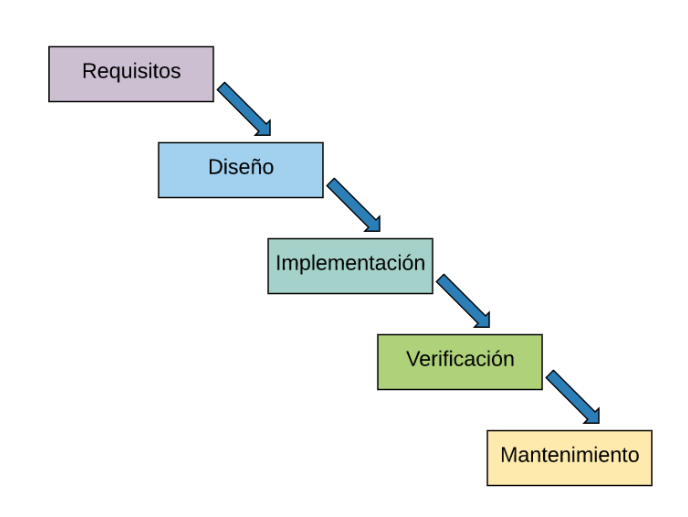
\includegraphics[width=0.4\columnwidth]{images/07/cascada.png}
   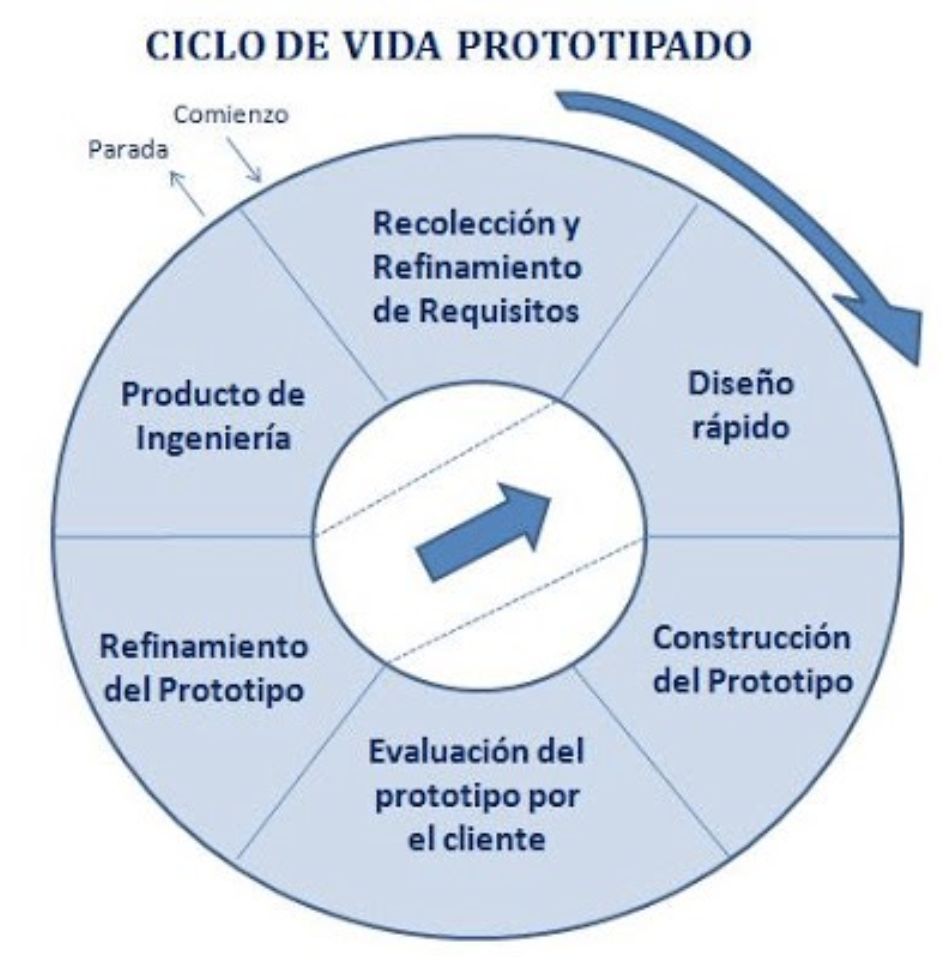
\includegraphics[width=0.4\columnwidth]{images/07/prototipado.png}\\
   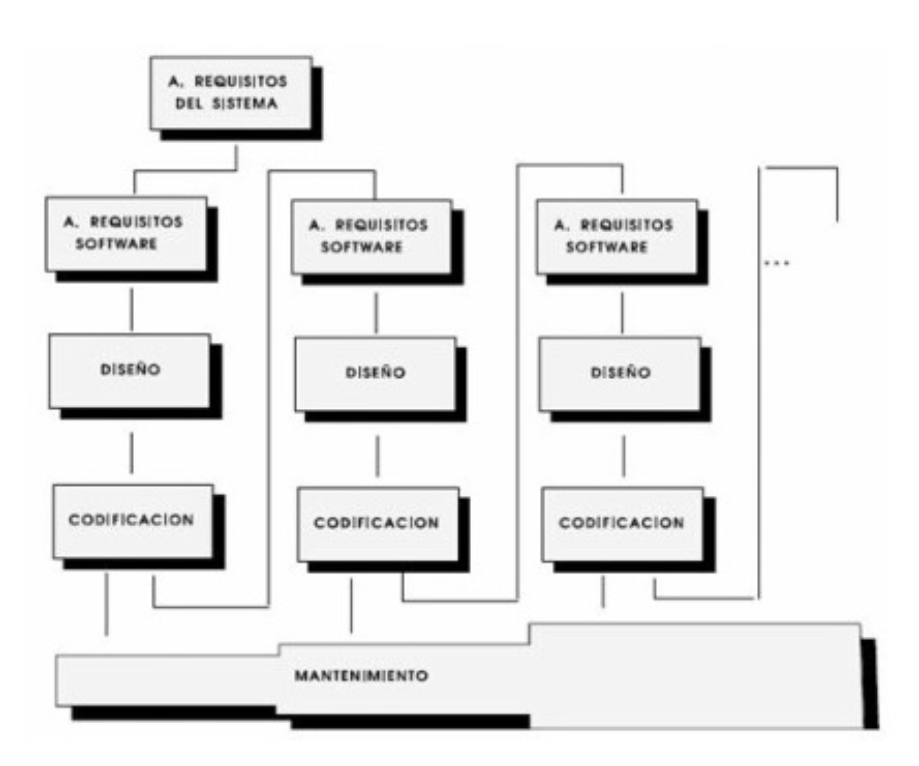
\includegraphics[width=0.4\columnwidth]{images/07/incremental.png}
   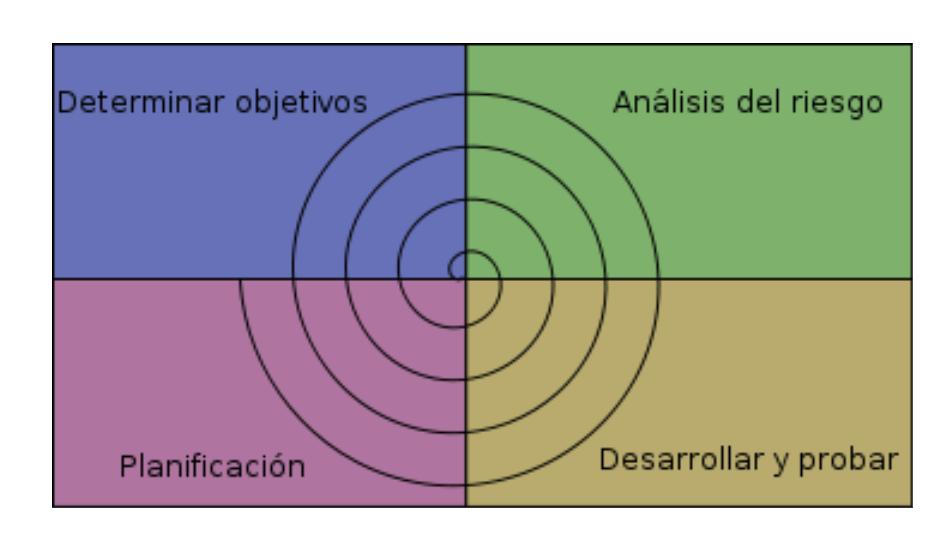
\includegraphics[width=0.4\columnwidth]{images/07/espiral.png}
   \caption{Enfoques generalistas: cascada, prototipado, incremental y espiral}
   \label{fig:enfoques}
\end{figure}

Un \ul{desarollo \textit{iterativo}} es aquel en el que, con cada entrega esperamos el feedback del usuario para decidir los siguientes pasos a seguir.
\nl

Un \ul{desarollo \textit{incremental}} es aquel en el que con cada entrega, tenemos acabada una pieza más del sistema.

Lo mejor es un \ul{desarollo \textit{iterativo} e \textit{incremental}}, que es aquel en el que cada entrega es una pieza del sistema, y además esperamos el feedback del usuario para decidir los siguientes pasos a seguir.

\section{Metodologías}

\begin{itemize}
   \item \textbf{Tradicionales} - Son orientadas al proyecto y presentan un enfoque lineal, con documentación formal.
   \begin{itemize}
   \item \textbf{RUP} (\textit{Rational Unified Process}) - Es un modelo incremental e iterativo que modela visualmente el software. Es un proceso dirigo por los casos de uso y centrado en la arquitectura\\
   \begin{figure}[htbp]
      \centering
      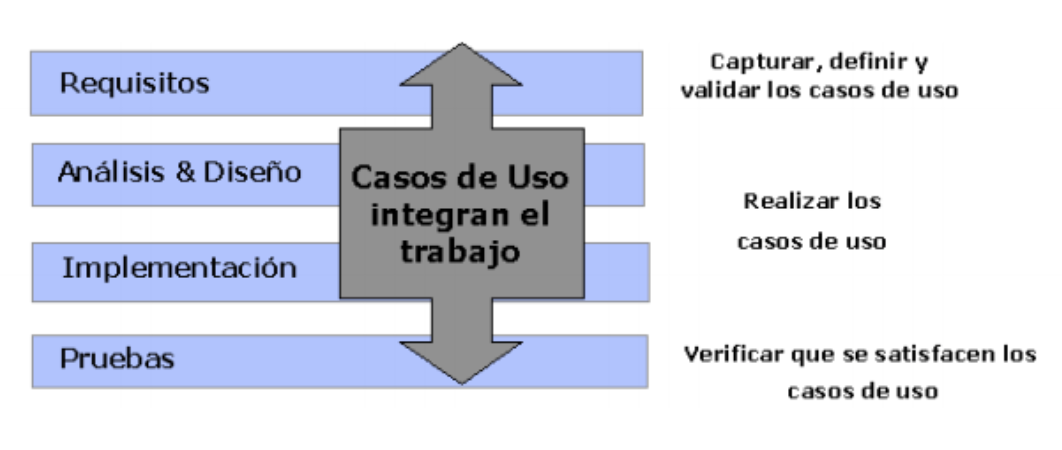
\includegraphics{images/07/rup.png}
      \caption{RUP schema}
      \label{fig:07/rup}
   \end{figure}

   \begin{paracol}{2}
      \colfill
      \item \textbf{V-Model} - Es un modelo de desarrollo de software que se basa en la idea de que cada fase del desarrollo debe tener una fase de prueba correspondiente. Se representa como una V, donde la parte izquierda representa las fases de desarrollo y la parte derecha representa las fases de prueba.\\
      No es muy flexible, requiere mucha\\ documientación, es muy orientada al proyecto, y es bueno por sistemas que son muy criticos cuando son apropiadas muchas pruebas, para comprobar la calidad del producto cada vez que se entrega una pieza.
      \colfill
      \switchcolumn
      \begin{figure}[htbp]
         \centering
         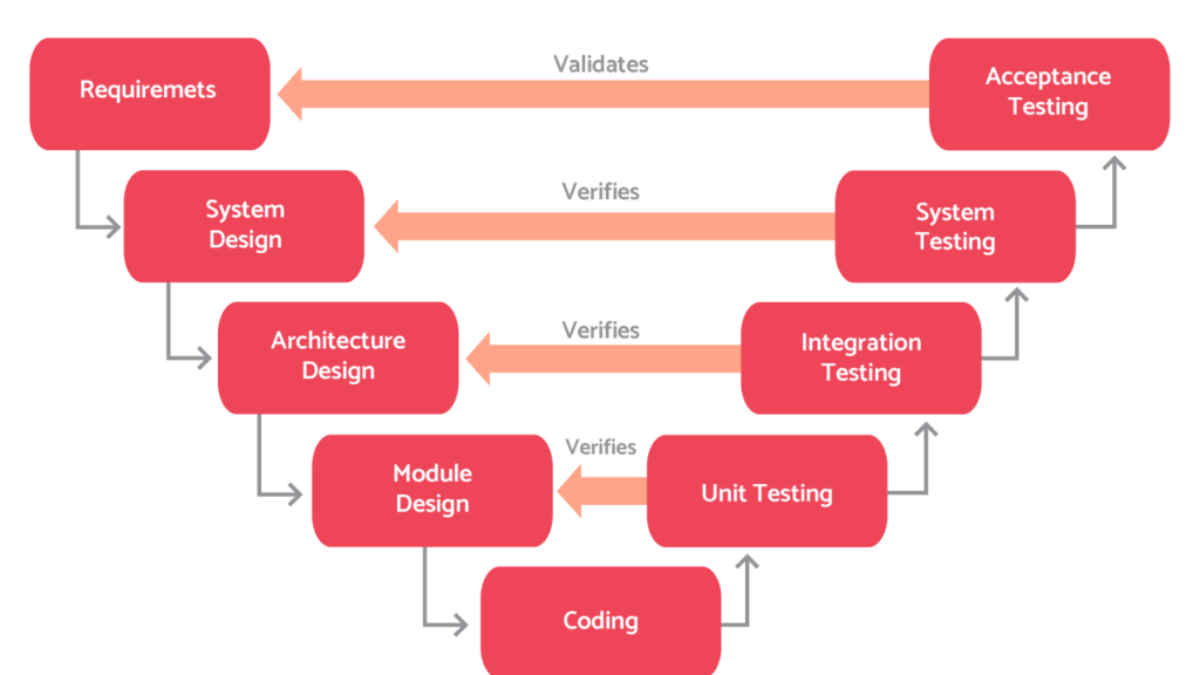
\includegraphics[width=0.99\columnwidth]{images/07/vmodel.png}
         \caption{V-Model}
         \label{fig:07/vmodel}
      \end{figure}
   \end{paracol}
   \end{itemize}
   \begin{paracol}{2}
      
   \item \textbf{Agile} - La palabra ``agile" se relaciona con la respuesta al progreso que pueden ofrecer las metodologías agiles.
    Las iteraciones son de 2-4 semanas, y la planificación se hace al finalizar cada iteración. Los valores del manifesto agile son:
   \note{\begin{itemize}[label=\textbullet]
      \item \textbf{Individuos e interacciones} sobre procesos y herramientas
      \item \textbf{Software funcionando} sobre documentación extensiva
      \item \textbf{Colaboración con el cliente} sobre negociación contractual
      \item \textbf{Respuesta al cambio} sobre seguir un plan
      \item \dots
   \end{itemize}}
   \vspace*{1em}
   \switchcolumn
   \colfill
   \begin{figure}[htbp]
      \centering
      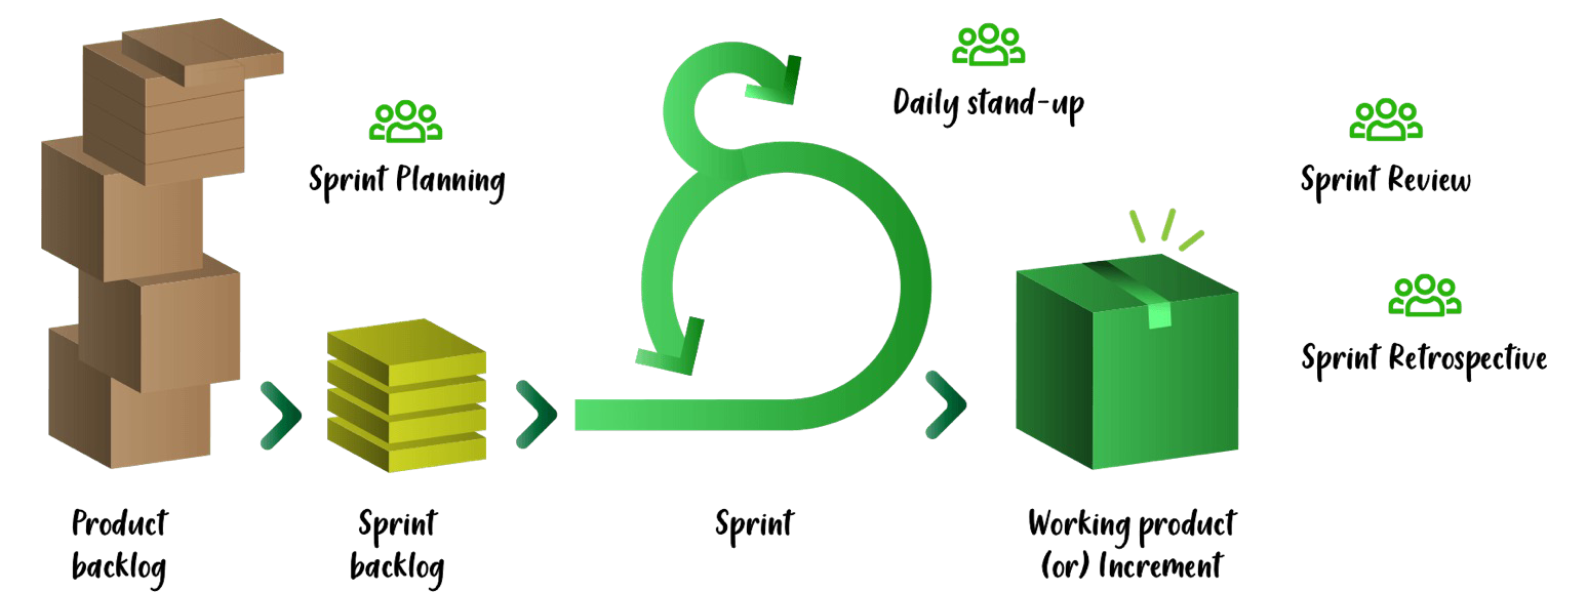
\includegraphics[width=0.99\columnwidth]{images/07/agile.png}
      \caption{Agile workflow}
      \label{fig:07/agile}
   \end{figure}
   \colfill
   \end{paracol}

   \newpage
   \begin{itemize}
      \item \textbf{Scrum} - Es un marco de trabajo ágil que se utiliza para gestionar proyectos de desarrollo de software. Se basa en la idea de que el desarrollo debe ser iterativo e incremental, y se centra en la colaboración entre los miembros del equipo.
      \begin{figure}[htbp]
         \centering
         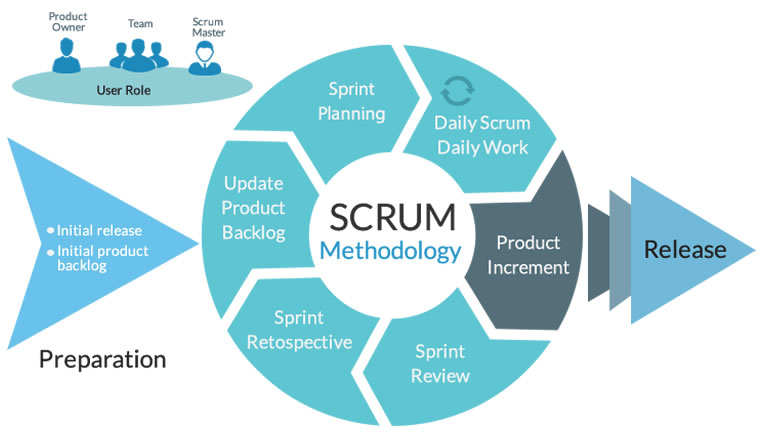
\includegraphics{images/07/scrum.jpg}
         \caption{Scrum framework}
         \label{fig:scrum}
      \end{figure}
      \item \textbf{Extreme Programming} - No tiene mucho diseño inicial, y entonces se va a hacer mucha refactorización.
   \end{itemize}
\end{itemize}

% // TODO

\section{Metodologías modernas}

{Características básicas de una estrategia de testing\ns
\begin{itemize}
	\item Proporciona feedback.
	\item Es rápida.
	\item Debe estar automatizada.
\end{itemize}}
Ejemplos modernós de metodologías son CI/CD (Integración continua y entrega continua) y DevOps.
\coolquote{El testing es una actividad integrada en el
desarrollo, no una fase posterior al desarrollo}{Manuela}
Las metodologías ágiles no ven al software testing como una fase separada, sino como \ul{parte integral del desarrollo de software al igual que la programación}.\\
Los equipos ágiles utilizan un enfoque de ``todo el equipo'' al testing, con la finalidad de integrar la calidad al desarrollo del producto, al contrario de un enfoque de primero fabricar el producto y luego inspeccionar para determinar su nivel de calidad

\newpage
\subsection{Test Driven Development (TDD)}

\begin{figure}[htbp]
   \centering
   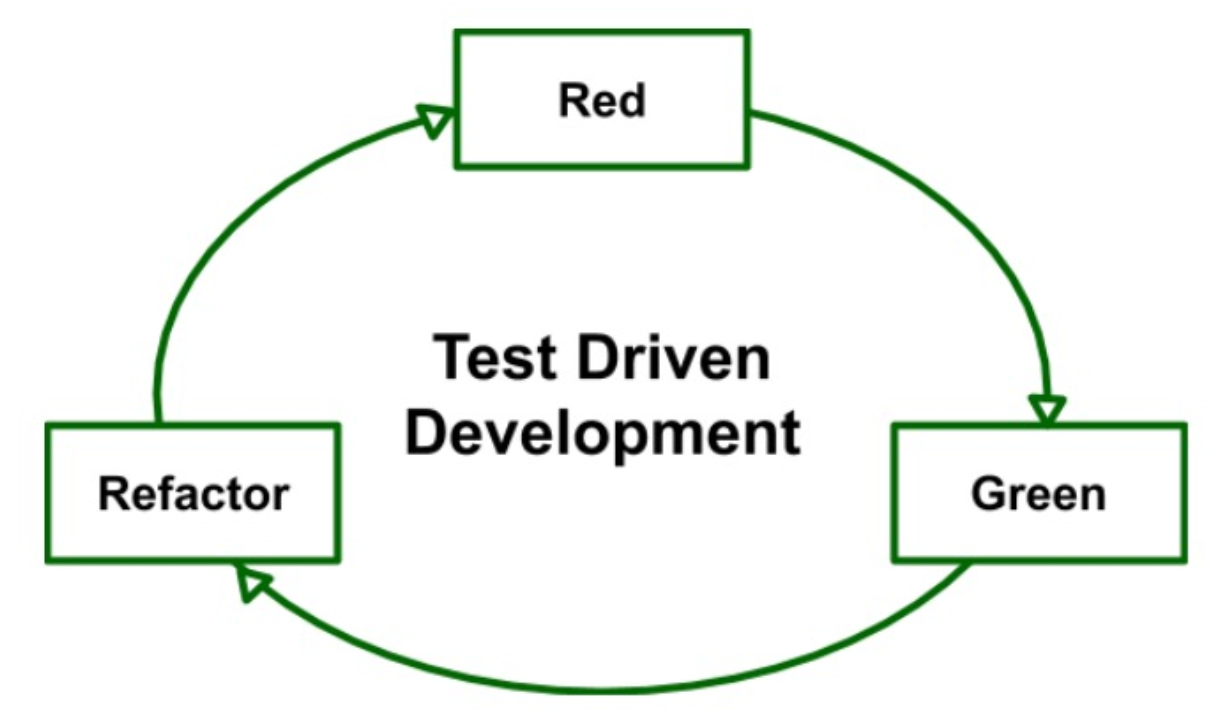
\includegraphics{images/07/tdd.png}
   \caption{TDD schema}
   \textred{\textit{``Red''}} significa que tenemos que escribir una prueba que falle, \textit{\color{green}``Green''} significa que tenemos que escribir el código necesario para hacer que la prueba pase, y \textit{``refactor''} significa que tenemos que refactorizar el código para mejorar su calidad, integrando el nuevo código con el antiguo.
   \label{fig:07/tdd}
\end{figure}

El \textit{Test Driven Development} (TDD)\footnote{Desarollo guiado por pruebas} es una metodología de desarrollo de software que se basa en la idea de que las pruebas deben ser escritas antes de escribir el código. El proceso de TDD se divide en tres pasos:
\begin{enumerate}
   \item Escribir una prueba que falle
   \item Escribir el código necesario para hacer que la prueba pase
   \item Refactorizar el código para mejorar su calidad
\end{enumerate}

\framedt{Reglas para el TDD}{
   \begin{enumerate}
      \item No está permitido escribir código de producción sin una prueba que falle
      \item No está permitido escribir más código de producción del necesario para hacer que la prueba pase
      \item No está permitido escribir más pruebas de las necesarias para cubrir el código de producción
   \end{enumerate}
}